\documentclass{article}
\title{im2col 实现原理详解}
\author{QwanxingxuA}
\usepackage{amsmath}
\usepackage{amssymb}
\usepackage{ctex}
\usepackage{graphicx}
\usepackage{listings}
\usepackage{float}
\usepackage{xcolor}
% 代码高亮设置
\lstset{
    language=Python,
    basicstyle=\ttfamily\small, 
    frame=single,        
    numbers=none,         
    breaklines=true,      
    tabsize=4,
    showstringspaces=false,
    keywordstyle=\color{blue},
    commentstyle=\color{gray}
}

\begin{document}
\maketitle

im2col 是卷积神经网络中经典的卷积加速方案：将卷积运算通过张量维度重排，转换成标准稠密矩阵乘法，从而可以调用CPU/GPU高度优化的BLAS矩阵计算库，大幅提升卷积运算速度。
该函数代码简短，但张量维度映射、行列排布逻辑极易混淆，下文结合源码与维度变换逐层拆解原理。

\section{基础实现代码}
\begin{lstlisting}
import numpy as np

def im2col(input_data, filter_h, filter_w, stride=1, pad=0):
    # 输入维度：N(批量数), C(通道数), H(输入特征图高), W(输入特征图宽)
    N, C, H, W = input_data.shape
    # 卷积输出特征图尺寸计算公式
    out_h = (H + 2 * pad - filter_h) // stride + 1
    out_w = (W + 2 * pad - filter_w) // stride + 1

    # 边界补零padding，仅在H、W维度上下左右填充
    img = np.pad(input_data, [(0,0), (0,0), (pad,pad), (pad,pad)], mode='constant')
    # 中间缓存张量：[N, C, fh, fw, out_h, out_w]
    col = np.zeros((N, C, filter_h, filter_w, out_h, out_w))

    # 遍历卷积核在空间维度上的每一个偏移位置
    for y in range(filter_h):
        y_end = y + stride * out_h
        for x in range(filter_w):
            x_end = x + stride * out_w
            # 按步长截取所有输出位置对应的图像窗口
            col[:, :, y, x, :, :] = img[:, :, y:y_end:stride, x:x_end:stride]

    # 维度置换 + 展平：最终形状 [N*out_h*out_w, C*filter_h*filter_w]
    col = col.transpose(0, 4, 5, 1, 2, 3).reshape(N * out_h * out_w, -1)
    return col
\end{lstlisting}

\section{参数符号定义}
\begin{table}[htbp]
    \centering
    \begin{tabular}{l l}
        \hline
        符号 & 含义说明 \\
        \hline
        $N$ & 批量样本数量（batch size） \\
        \hline
        $C$ & 输入特征图通道数 \\
        \hline
        $F_H$ & 卷积核高度 \\
        \hline
        $F_W$ & 卷积核宽度 \\
        \hline
        $O_H$ & 卷积输出特征图高度 \\
        \hline
        $O_W$ & 卷积输出特征图宽度 \\
        \hline
        $K$ & 卷积核总个数（输出通道数） \\
        \hline
    \end{tabular}
\end{table}

\section{维度变换核心逻辑}
1. 填充后的图像张量 \(\boldsymbol{img}\) 依旧保有原图空间结构，仅边界扩充零元素，数据语义未发生改变；
2. 张量 \(\boldsymbol{col}\) 的作用：枚举卷积滑动过程中，**每一个卷积窗口会覆盖到的所有图像像素**。
    卷积核尺寸维度：\(\boldsymbol{Kernel}\in \mathbb{R}^{C\times F_H\times F_W}\)
    单个卷积窗口对应空间采样位置总数：\(N\times O_H\times O_W\)

将两个维度耦合排布：
\[
\text{col张量维度} = \big(N,O_H,O_W\big) \times \big(C,F_H,F_W\big)
\]
前半部分：所有需要计算卷积的空间位置；后半部分：单个卷积核完整权重向量长度。

将卷积核集合展开为二维权重矩阵：
卷积核群整体维度 \(K\times C F_H F_W\)，转置后得到 \(\boldsymbol{W}^T \in \mathbb{R}^{C F_H F_W \times K}\)。

此时卷积运算等价于矩阵乘法：
\[
\boldsymbol{Output} = \boldsymbol{col} \cdot \boldsymbol{W}^T
\]
- \(\boldsymbol{col}\in \mathbb{R}^{N O_H O_W \times C F_H F_W}\)
- 结果维度：\(N O_H O_W \times K\)
最后只需将结果reshape还原为四维张量 \((N,K,O_H,O_W)\)，即为标准卷积输出特征图。

\section{本质思想总结}
1. im2col没有压缩或扩充存储空间，只是把卷积滑动窗口逐行摊平，将局部邻域运算重构为全局矩阵乘；
2. 卷积的数学定义就是：卷积核权重与感受野像素逐元素相乘后求和，恰好对应矩阵乘法中行向量与列向量的点积运算；
3. 
    优势：复用高度优化的通用矩阵乘法(GEMM)库，CPU/GPU加速效果极佳；
    缺点：会产生大量冗余复制的像素数据，显存/内存占用显著上升。

\begin{figure}[H]
    \centering
    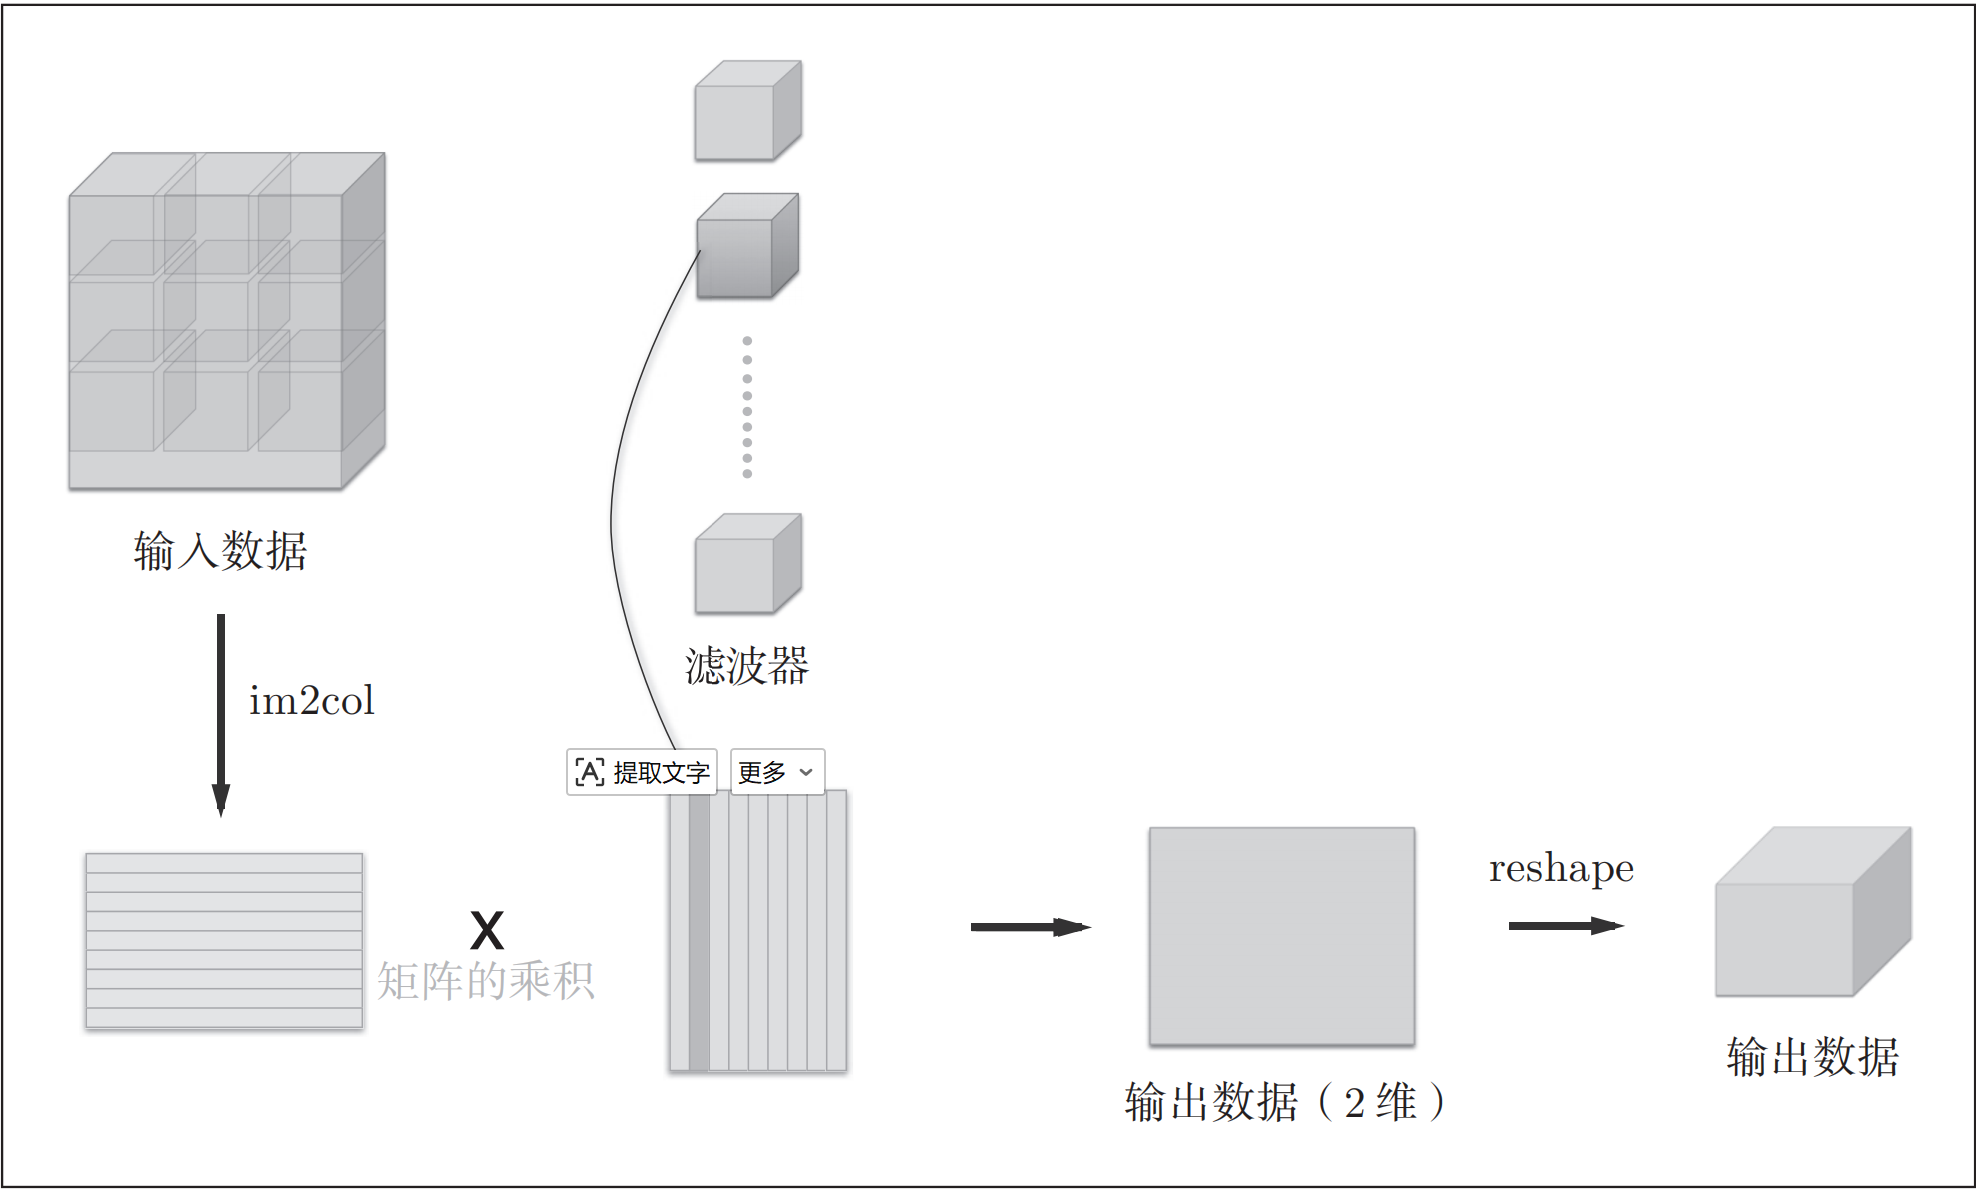
\includegraphics[width=0.8\textwidth]{im2col.png}
    \caption{im2col卷积窗口摊平可视化示意图}
\end{figure}

\end{document}